\documentclass[10pt, aspectratio=169]{beamer}

% =========================================================
% 1. THEME & PACKAGES SETUP (FIX TRIỆT ĐỂ FONT T5 & BEAMER)
% =========================================================
\usetheme{Madrid}
\usecolortheme{whale}
\usefonttheme{professionalfonts}

\usepackage[T5,T1]{fontenc}
\usepackage[utf8]{vietnam}
\usepackage{lmodern}
% Ánh xạ font nghiêng T5/cmss/m/it sang T5/cmss/m/sl để diệt vĩnh viễn lỗi font Beamer
\DeclareFontShape{T5}{cmss}{m}{it}{<->sub*cmss/m/sl}{}

\usepackage{amsmath, amsfonts, amssymb}
\usepackage{graphicx}
\usepackage{booktabs}
\usepackage{tabularx}
\usepackage{tikz}
\usetikzlibrary{positioning, shadows, shapes.geometric, arrows.meta}

% =========================================================
% 2. COLOR PALETTE DEFINITION (PROFESSIONAL BEAMER)
% =========================================================
\definecolor{primaryblue}{RGB}{24, 76, 120}    % Màu chủ đạo (Deep Navy Blue)
\definecolor{accentorange}{RGB}{235, 130, 60}  % Màu nhấn (Warm Orange)
\definecolor{darknavy}{RGB}{15, 45, 75}        % Thẻ khối thứ 3 (Dark Navy)
\definecolor{lightbg}{RGB}{245, 247, 250}      % Nền khối thông tin (Soft Gray/Blue)

\setbeamercolor{palette primary}{bg=primaryblue, fg=white}
\setbeamercolor{palette secondary}{bg=primaryblue!90, fg=white}
\setbeamercolor{palette tertiary}{bg=darknavy, fg=white}
\setbeamercolor{titlelike}{parent=palette primary}
\setbeamercolor{structure}{fg=primaryblue}

% Tùy chỉnh màu sắc hệ thống Block của Beamer
\setbeamercolor{block title}{bg=primaryblue, fg=white}
\setbeamercolor{block body}{bg=lightbg, fg=black}
\setbeamercolor{block title alert}{bg=accentorange, fg=white}
\setbeamercolor{block body alert}{bg=lightbg, fg=black}
\setbeamercolor{block title example}{bg=darknavy, fg=white}
\setbeamercolor{block body example}{bg=lightbg, fg=black}

% Cấu hình thanh điều hướng & Footer sạch sẽ
\setbeamertemplate{navigation symbols}{}
\setbeamertemplate{footline}[frame number]

% =========================================================
% 3. PRESENTATION METADATA
% =========================================================
\title[SLRMS - AI Search \& RAG System]{HỆ THỐNG QUẢN LÝ TÀI LIỆU HỌC TẬP THÔNG MINH\\ TÍCH HỢP HYBRID SEARCH \& CHAT RAG}
\subtitle{Báo cáo Tiến độ / Báo cáo Nghiệm thu Thực tập}
\date{\today}

\begin{document}

% =========================================================
% SLIDE 1: TITLE PAGE (2-COLUMN GRID TỐI ƯU)
% =========================================================
\begin{frame}[plain]
    \vfill
    \begin{center}
        \begin{beamercolorbox}[sep=8pt,center,rounded=true,shadow=true]{palette primary}
            {\large \textbf{SMART LEARNING RESOURCE MANAGEMENT SYSTEM (SLRMS)}}\\[0.1cm]
        \end{beamercolorbox}
        \vspace{0.15cm}
        {\footnotesize \textit{Báo cáo Nghiệm thu Thực tập Doanh nghiệp}}
    \end{center}

    \vspace{0.15cm}
    
    \begin{beamercolorbox}[sep=5pt,rounded=true]{block body}
        \footnotesize
        \begin{columns}[T]
            \begin{column}{0.48\textwidth}
                \textbf{\textcolor{primaryblue}{Sinh viên thực hiện:}}
                \begin{itemize}
                    \item Tạ Văn Nghĩa -- 23000145 -- K68A2 Toán tin
                    \item Trần Viết Kiên -- 23000132 -- K68A2 Toán tin
                    \item Mạc Văn Tường -- 23001951 -- K68A4 KHMT\&TT
                    \item Đinh Quang Tiến -- 23001943 -- K68A4 KHMT\&TT
                \end{itemize}
            \end{column}
            
            \begin{column}{0.48\textwidth}
                \textbf{\textcolor{primaryblue}{\phantom{Sinh viên thực hiện:}}}
                \begin{itemize}
                    \item Đoàn Thị Minh Khuê -- 23001894 -- K68A4 KHMT\&TT
                    \item Bùi Quang Chiến -- 23001837 -- K68A3 KHMT\&TT
                    \item Văn Việt Quang -- 23000152 -- K68A2 Toán tin
                    \item Bùi Phúc Bình -- 23021478 -- K68-I\_CS4
                \end{itemize}
            \end{column}
        \end{columns}
        
        \vspace{0.08cm}
        \centering
        \textcolor{primaryblue}{\rule{0.9\textwidth}{0.4pt}}\\[0.08cm]
        \textbf{Người hướng dẫn}: \textbf{Hồ Trọng Hải}
    \end{beamercolorbox}
    \vfill
\end{frame}

% =========================================================
% SLIDE 2: AGENDA
% =========================================================
\begin{frame}{Nội dung trình bày}
    \tableofcontents
\end{frame}

% =========================================================
% ĐẦU MỤC 1: GIỚI THIỆU DỰ ÁN
% =========================================================
\section{Giới thiệu dự án}

\begin{frame}{1. Bài toán và mục tiêu của dự án}
    \begin{block}{Bài toán Đặt ra}
        Kho tài liệu học tập lớn nhưng rời rạc $\rightarrow$ Cần giải pháp Web tập trung vừa quản lý học liệu chuẩn hóa, vừa tích hợp AI hỗ trợ khai thác tri thức thông minh.
    \end{block}

    \vspace{0.15cm}

    \begin{columns}[T]
        \begin{column}{0.48\textwidth}
            \begin{alertblock}{Sprint 1: Phân hệ Cốt lõi (MVP)}
                \begin{itemize}
                    \item \textbf{Auth JWT \& RBAC:} Đăng ký, đăng nhập JWT, phân quyền 3 vai trò (Admin, Teacher, Student).
                    \item \textbf{Tài liệu \& Thư mục:} Upload file, cây thư mục phân cấp Môn học $\rightarrow$ Chủ đề.
                    \item \textbf{Search \& Social:} Tìm kiếm từ khóa, Bookmark, Comment, Rating \& Dashboard.
                \end{itemize}
            \end{alertblock}
        \end{column}

        \begin{column}{0.48\textwidth}
            \begin{exampleblock}{Sprint 2: Tính năng AI Mở rộng}
                \begin{itemize}
                    \item \textbf{Trợ lý AI Chat RAG:} Tích hợp Gemini LLM, trích dẫn nguồn, Chat Sessions độc lập.
                    \item \textbf{Tự động Tóm tắt AI:} Trích xuất \& sinh bản tóm tắt nội dung ngắn gọn.
                    \item \textbf{Sinh 3 Câu hỏi Gợi ý:} Tự động khởi tạo câu hỏi trọng tâm giúp tra cứu nhanh.
                \end{itemize}
            \end{exampleblock}
        \end{column}
    \end{columns}
\end{frame}

% =========================================================
% ĐẦU MỤC 2: CÔNG NGHỆ VÀ CÔNG CỤ SỬ DỤNG
% =========================================================
\section{Công nghệ và công cụ sử dụng}

\begin{frame}{2. Stack công nghệ sử dụng}
    \begin{table}
        \centering
        \small
        \renewcommand{\arraystretch}{1.2}
        \begin{tabularx}{\textwidth}{>{\bfseries\color{primaryblue}}p{3.2cm} X X}
            \toprule
            \textbf{\textcolor{primaryblue}{Công nghệ}} & \textbf{\textcolor{primaryblue}{Ưu điểm Cốt lõi}} & \textbf{\textcolor{primaryblue}{Thách thức / Hạn chế}} \\
            \midrule
            FastAPI (Python) & Tốc độ cao, Swagger UI tự động, sẵn \texttt{BackgroundTasks} & Cần tự thiết kế kiến trúc phân tầng \\
            \addlinespace[0.05cm]
            PostgreSQL \& \texttt{pgvector} & CSDL quan hệ + Vector Search 384d tập trung duy nhất & Cần chiến lược Index khi dữ liệu lớn \\
            \addlinespace[0.05cm]
            Next.js 14 \& React & App Router, TypeScript, giao diện SPA mượt mà & Xử lý State phức tạp ở luồng Chat AI \\
            \addlinespace[0.05cm]
            Redis Service & Quản lý Refresh Token Session \& thu hồi Logout & Phụ thuộc thêm 1 dịch vụ memory cache \\
            \addlinespace[0.05cm]
            Docker \& Compose & Đóng gói 1-Click toàn vẹn, tự động Alembic Migration & Tiêu tốn tài nguyên máy chủ ở Local \\
            \bottomrule
        \end{tabularx}
        \caption{Bảng tổng hợp tinh gọn Ưu \& Nhược điểm Stack Công nghệ Hệ thống}
    \end{table}
\end{frame}

% =========================================================
% ĐẦU MỤC 3: KIẾN TRÚC VÀ CÁC TÍNH NĂNG CHÍNH
% =========================================================
\section{Kiến trúc và các tính năng chính}

\begin{frame}{3.1 Kiến trúc Tổng thể Hệ thống (Client-Server)}
    \begin{center}
        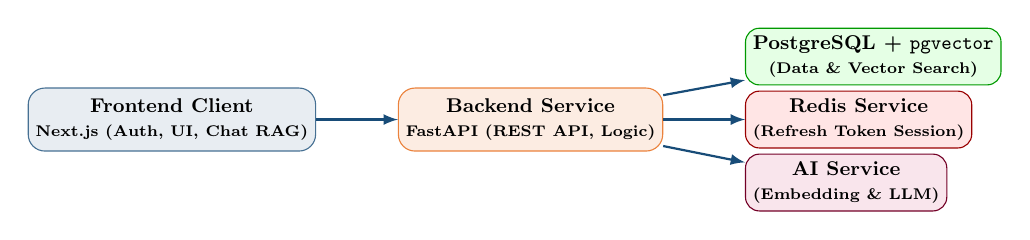
\begin{tikzpicture}[
            scale=0.8, transform shape,
            node distance=1.0cm and 1.3cm,
            box/.style={draw=primaryblue!80, fill=primaryblue!10, rounded corners=6pt, minimum width=3.2cm, minimum height=1.0cm, align=center, font=\bfseries\small},
            orangebox/.style={draw=accentorange, fill=accentorange!15, rounded corners=6pt, minimum width=3.5cm, minimum height=1.0cm, align=center, font=\bfseries\small},
            greenbox/.style={draw=green!60!black, fill=green!10, rounded corners=5pt, minimum width=2.8cm, minimum height=0.8cm, align=center, font=\bfseries\small},
            redbox/.style={draw=red!60!black, fill=red!10, rounded corners=5pt, minimum width=2.8cm, minimum height=0.8cm, align=center, font=\bfseries\small},
            purplebox/.style={draw=purple!60!black, fill=purple!10, rounded corners=5pt, minimum width=2.8cm, minimum height=0.8cm, align=center, font=\bfseries\small},
            arrow/.style={-latex, thick, primaryblue}
        ]
            \node[box] (ui) {Frontend Client\\{\scriptsize Next.js (Auth, UI, Chat RAG)}};
            \node[orangebox, right=of ui] (api) {Backend Service\\{\scriptsize FastAPI (REST API, Logic)}};
            
            \node[greenbox, right=of api, yshift=1.0cm] (db) {PostgreSQL + \texttt{pgvector}\\{\scriptsize (Data \& Vector Search)}};
            \node[redbox, right=of api] (redis) {Redis Service\\{\scriptsize (Refresh Token Session)}};
            \node[purplebox, right=of api, yshift=-1.0cm] (ai) {AI Service\\{\scriptsize (Embedding \& LLM)}};

            \draw[arrow] (ui) -- (api);
            \draw[arrow] (api) -- (db);
            \draw[arrow] (api) -- (redis);
            \draw[arrow] (api) -- (ai);
        \end{tikzpicture}
    \end{center}

    \vspace{0.1cm}
    \begin{itemize}
        \item \textbf{Phân tách Độc lập:} Frontend không truy cập trực tiếp CSDL hay AI Service.
        \item \textbf{Backend Điều phối Tập trung:} Đảm bảo Auth, phân quyền RBAC \& nghiệp vụ trước khi trả dữ liệu.
    \end{itemize}
\end{frame}

\begin{frame}{3.2 Kiến trúc Backend Phân tầng (Layered Architecture)}
    \begin{center}
        \begin{tikzpicture}[
            scale=0.8, transform shape,
            node distance=0.4cm and 0.8cm,
            layer/.style={draw=primaryblue!80, fill=primaryblue!8, rounded corners=5pt, minimum width=10.5cm, minimum height=0.75cm, align=center, font=\bfseries\small},
            arrow/.style={-latex, thick, primaryblue}
        ]
            \node[layer] (l1) {\textcolor{primaryblue}{API Layer} -- HTTP, Validation, Authentication, Authorization (\texttt{api/routers})};
            \node[layer, below=0.4cm of l1] (l2) {\textcolor{primaryblue}{Service Layer} -- Business Logic \& Điều phối thành phần (\texttt{services})};
            \node[layer, below=0.4cm of l2] (l3) {\textcolor{primaryblue}{Repository Layer} -- Data Access đóng gói qua SQLAlchemy (\texttt{repositories})};
            \node[layer, below=0.4cm of l3, fill=green!10, draw=green!60!black] (l4) {\textcolor{green!50!black}{Data Layer} -- PostgreSQL + \texttt{pgvector} (\texttt{models})};

            \draw[arrow] (l1) -- (l2);
            \draw[arrow] (l2) -- (l3);
            \draw[arrow] (l3) -- (l4);
        \end{tikzpicture}
    \end{center}

    \vspace{0.1cm}
    \begin{itemize}
        \item \textbf{Luồng 1 chiều nghiêm ngặt:} \textbf{API Layer $\rightarrow$ Service Layer $\rightarrow$ Repository Layer $\rightarrow$ Data Layer}.
        \item \textbf{Loose Coupling:} Tách biệt xử lý nghiệp vụ khỏi CSDL qua SQLAlchemy ORM.
    \end{itemize}
\end{frame}

\begin{frame}[t]{3.3 Thiết kế Cơ sở Dữ liệu \& Vector Search}
    \footnotesize
    \begin{columns}[T,onlytextwidth]
        \begin{column}{0.485\textwidth}
            \begin{block}{Kiến trúc CSDL Hybrid}
                \begin{itemize}
                    \setlength{\itemsep}{2pt}
                    \setlength{\parskip}{0pt}
                    \item \textbf{PostgreSQL Engine:} Lưu user, folder, document \& tương tác xã hội.
                    \item \textbf{Extension \texttt{pgvector}:} Lưu kiểu \texttt{vector(384)} tại \texttt{document\_chunks} phục vụ RAG.
                    \item \textbf{Ưu điểm:} Cùng 1 CSDL cho cả Quan hệ \& Vector Search.
                \end{itemize}
            \end{block}

            \vspace{-0.05cm}
            \begin{exampleblock}{Schema Migration}
                \begin{itemize}
                    \setlength{\itemsep}{2pt}
                    \setlength{\parskip}{0pt}
                    \item \textbf{Alembic Versioning:} Quản lý thay đổi CSDL trực tiếp trong code.
                    \item \textbf{Docker Automation:} Tự động \texttt{upgrade head} trước khi backend chạy.
                \end{itemize}
            \end{exampleblock}
        \end{column}

        \hfill

        \begin{column}{0.485\textwidth}
            \begin{alertblock}{Mô hình ERD (12 Bảng CSDL)}
                \begin{itemize}
                    \setlength{\itemsep}{2pt}
                    \setlength{\parskip}{0pt}
                    \item \textbf{Tài liệu \& Thư mục (5):} \texttt{users}, \texttt{folders}, \texttt{documents}, \texttt{tags}, \texttt{document\_tags}.
                    \item \textbf{Tương tác Xã hội (3):} \texttt{bookmarks}, \texttt{comments}, \texttt{ratings}.
                    \item \textbf{AI RAG \& Auth (4):} \texttt{document\_chunks}, \texttt{chat\_sessions}, \texttt{chat\_messages}, \texttt{password\_reset\_tokens}.
                \end{itemize}
            \end{alertblock}

            \vspace{-0.05cm}
            \begin{beamercolorbox}[sep=4pt, rounded=true]{block body}
                \scriptsize
                \textbf{\textcolor{primaryblue}{Chính sách Ràng buộc Toàn vẹn:}}
                \begin{itemize}
                    \setlength{\itemsep}{1pt}
                    \setlength{\parskip}{0pt}
                    \item Xóa document $\rightarrow$ xóa dây chuyền chunks, bookmarks, comments, ratings.
                    \item Xóa folder $\rightarrow$ giữ nguyên tài liệu, ngắt liên kết \texttt{folder\_id}.
                \end{itemize}
            \end{beamercolorbox}
        \end{column}
    \end{columns}
\end{frame}

\begin{frame}{3.4 Phân hệ Xác thực JWT \& Quản lý Thư mục Cây}
    \begin{columns}[T]
        \begin{column}{0.48\textwidth}
            \begin{block}{Xác thực JWT \& Phân quyền RBAC}
                \begin{itemize}
                    \item \textbf{JWT Token:} Access Token ngắn hạn + Refresh Token Rotation quản lý trên Redis.
                    \item \textbf{Mô hình RBAC 3 vai trò:} ADMIN, TEACHER, STUDENT với dependency \texttt{require\_role}.
                    \item \textbf{Bảo mật:} Băm bcrypt, khôi phục mật khẩu SHA-256 token dùng 1 lần, thu hồi session khi logout.
                \end{itemize}
            \end{block}
        \end{column}

        \begin{column}{0.48\textwidth}
            \begin{alertblock}{Tổ chức Cây Thư mục Đa cấp}
                \begin{itemize}
                    \item \textbf{Self-referencing Tree:} \texttt{parent\_folder\_id} trỏ chính mình (Môn học $\rightarrow$ Chương $\rightarrow$ Chủ đề).
                    \item \textbf{Cô lập Dữ liệu:} Thuộc tính \texttt{owner\_id} cô lập độc lập cây thư mục Giáo viên.
                    \item \textbf{Xóa An toàn:} Khóa ngoại \texttt{ON DELETE SET NULL} ngắt liên kết, bảo toàn file.
                \end{itemize}
            \end{alertblock}
        \end{column}
    \end{columns}
\end{frame}

\begin{frame}{3.5 Phân hệ Quản lý Tài liệu, Xử lý Nền \& Tương tác}
    \begin{columns}[T]
        \begin{column}{0.48\textwidth}
            \begin{block}{Quản lý Tài liệu \& Xử lý Nền}
                \begin{itemize}
                    \item \textbf{Upload Không Chặn:} Trả \texttt{201 Created} (\texttt{PENDING}) tức thì cho Client.
                    \item \textbf{FastAPI \texttt{BackgroundTasks}:} Tiến trình ngầm extract, chunk, nhúng vector 384d \& summary $\rightarrow$ \texttt{DONE}.
                    \item \textbf{Runtime Calculation:} Tính \texttt{file\_size} từ tệp vật lý lúc gọi API; gán tên file tải về thân thiện.
                \end{itemize}
            \end{block}
        \end{column}

        \begin{column}{0.48\textwidth}
            \begin{exampleblock}{Tương tác Xã hội \& Thống kê}
                \begin{itemize}
                    \item \textbf{Bookmark cá nhân:} Lưu danh sách tài liệu cá nhân yêu thích.
                    \item \textbf{Comment \& Rating:} Bình luận theo thời gian \& Đánh giá 1-5 sao trung bình.
                    \item \textbf{Dashboard Thống kê:} Biểu đồ lượt tải theo ngày, phân bố thư mục \& vai trò user.
                \end{itemize}
            \end{exampleblock}
        \end{column}
    \end{columns}
\end{frame}

\begin{frame}{3.6 Các Tính năng Mở rộng Tích hợp AI}
    \begin{columns}[T]
        \begin{column}{0.48\textwidth}
            \begin{block}{Trợ lý AI Hỏi đáp (RAG Chatbot)}
                \begin{itemize}
                    \item \textbf{Tích hợp LLMs:} Gemini 2.5/OpenAI với cơ chế Top-K Context Retrieval (K=5).
                    \item \textbf{Trích dẫn Nguồn (\texttt{citations}):} Kèm tên file \& trang tài liệu tham chiếu; từ chối khi thiếu căn cứ.
                    \item \textbf{Chat Sessions:} Quản lý phiên trò chuyện độc lập cho từng tài liệu.
                \end{itemize}
            \end{block}
        \end{column}

        \begin{column}{0.48\textwidth}
            \begin{alertblock}{Tự động Tóm tắt \& Sinh Câu hỏi AI}
                \begin{itemize}
                    \item \textbf{Tóm tắt Tự động:} Trích xuất \& sinh bản tóm tắt nội dung ngắn gọn.
                    \item \textbf{Sinh Câu hỏi Gợi ý:} Phân tích ngữ cảnh tự động khởi tạo 3 câu hỏi trọng tâm.
                    \item \textbf{Smart Fallback:} Dự phòng linh hoạt không phụ thuộc API Key bên thứ ba.
                \end{itemize}
            \end{alertblock}
        \end{column}
    \end{columns}
\end{frame}

% =========================================================
% ĐẦU MỤC 4: THÁCH THỨC KỸ THUẬT
% =========================================================
\section{Thách thức và giải pháp}

\begin{frame}{4.1 Thách thức 1: Xử lý Tác vụ AI Nặng Chạy Nền Không Chặn API}
    \begin{block}{Hiện trạng Sự cố}
        Trích xuất văn bản, cắt nhỏ, nhúng vector 384d và sinh tóm tắt AI tốn thời gian $\rightarrow$ Xử lý đồng bộ gây treo/nghẽn API chính.
    \end{block}

    \vspace{0.15cm}
    \begin{alertblock}{Giải pháp Kỹ thuật Triển khai}
        Kiến trúc \textbf{Non-blocking API \& Background Processing}:
        \begin{itemize}
            \item \textbf{Phản hồi Tức thì:} Backend tạo bản ghi \texttt{PENDING} và trả phản hồi \texttt{201 Created} ngay cho Client.
            \item \textbf{FastAPI \texttt{BackgroundTasks}:} Đẩy toàn bộ luồng xử lý AI nặng xuống tiến trình ngầm bất đồng bộ.
            \item \textbf{Cập nhật Trạng thái Động:} Tiến trình ngầm tự đọc file, trích xuất, nhúng vector, tóm tắt $\rightarrow$ \texttt{DONE} / \texttt{FAILED}.
        \end{itemize}
    \end{alertblock}
\end{frame}

\begin{frame}{4.2 Thách thức 2: Ngăn Chu trình Cây Thư mục \& Bảo toàn Dữ liệu}
    \begin{block}{Hiện trạng Sự cố}
        Trong cấu trúc tự tham chiếu, di chuyển thư mục cha vào thư mục con tạo chu trình vô tận; nguy cơ mất tài liệu khi xóa thư mục.
    \end{block}

    \vspace{0.15cm}
    \begin{alertblock}{Giải pháp Kỹ thuật Triển khai}
        Thuật toán \textbf{\texttt{subtree\_ids} Stack \& Khóa ngoại Safe Delete}:
        \begin{itemize}
            \item \textbf{Duyệt Cây Ngăn Chu trình:} Dùng Stack \& tập \texttt{visited} lấy ID cây con; từ chối 100\% di chuyển vào cây con.
            \item \textbf{Kế thừa Môn học:} Tự động đồng bộ thuộc tính môn học cho toàn bộ cây con.
            \item \textbf{Bảo toàn Tài liệu:} Xóa thư mục chỉ ngắt \texttt{folder\_id}, bảo toàn 100\% tệp tin và metadata tài liệu.
        \end{itemize}
    \end{alertblock}
\end{frame}

% =========================================================
% ĐẦU MỤC 5: HÌNH ẢNH SẢN PHẨM & DEMO GIAO DIỆN & KIỂM THỬ
% =========================================================
\section{Hình ảnh sản phẩm và Kiểm thử}

\begin{frame}{5.1 Sản phẩm Đạt được \& Giao diện Người dùng}
    \begin{columns}[T]
        \begin{column}{0.48\textwidth}
            \begin{block}{Sản phẩm Đạt được (Mục 3.1)}
                \begin{itemize}
                    \item \textbf{Đóng gói Docker Compose:} Khởi chạy toàn bộ 5 services với \texttt{docker compose up --build}.
                    \item \textbf{Vòng đời Complete:} JWT Auth/RBAC, Cây thư mục, AI Pipeline, Chat RAG.
                    \item \textbf{Tài liệu API Tự động:} Swagger UI (\texttt{/docs}), ReDoc \& OpenAPI JSON.
                \end{itemize}
            \end{block}
        \end{column}

        \begin{column}{0.48\textwidth}
            \begin{alertblock}{Bộ Giao diện Next.js (Mục 3.2)}
                \begin{itemize}
                    \item \textbf{Bao phủ 100\% Nghiệp vụ:} Auth, Dashboard, Document, Folder, Chat RAG, Bookmark, Admin.
                    \item \textbf{Trải nghiệm SPA:} App Router, TypeScript, giao diện hiện đại mượt mà.
                \end{itemize}
            \end{alertblock}
        \end{column}
    \end{columns}
\end{frame}

\begin{frame}{5.2 Demo Giao diện -- Tìm kiếm \& Chi tiết Tài liệu}
    \begin{columns}[T]
        \begin{column}{0.48\textwidth}
            \begin{block}{1. Giao diện Tìm kiếm Tài liệu}
                \centering
                \IfFileExists{search_ui.png}{
                    \includegraphics[width=\textwidth, height=3.6cm, keepaspectratio]{search_ui.png}
                }{
                    \vspace{0.8cm}
                    \small \textit{[Up ảnh \texttt{search\_ui.png} lên Overleaf]}
                    \vspace{0.8cm}
                }
                \vspace{0.05cm}
                {\tiny Tìm kiếm từ khóa theo tiêu đề, thẻ (tag), môn học \& phân trang.}
            \end{block}
        \end{column}

        \begin{column}{0.48\textwidth}
            \begin{alertblock}{2. Chi tiết Tài liệu \& Tóm tắt AI}
                \centering
                \IfFileExists{doc_detail_ui.png}{
                    \includegraphics[width=\textwidth, height=3.6cm, keepaspectratio]{doc_detail_ui.png}
                }{
                    \vspace{0.8cm}
                    \small \textit{[Up ảnh \texttt{doc\_detail\_ui.png} lên Overleaf]}
                    \vspace{0.8cm}
                }
                \vspace{0.05cm}
                {\tiny Xem metadata, tóm tắt AI tự động \& câu hỏi gợi ý.}
            \end{alertblock}
        \end{column}
    \end{columns}
\end{frame}

\begin{frame}{5.3 Demo Giao diện -- Trợ lý Chat RAG \& Bookmark}
    \begin{columns}[T]
        \begin{column}{0.48\textwidth}
            \begin{block}{3. Trợ lý AI Hỏi đáp (RAG Chat Modal)}
                \centering
                \IfFileExists{rag_chat_ui.png}{
                    \includegraphics[width=\textwidth, height=3.6cm, keepaspectratio]{rag_chat_ui.png}
                }{
                    \vspace{0.8cm}
                    \small \textit{[Up ảnh \texttt{rag\_chat\_ui.png} lên Overleaf]}
                    \vspace{0.8cm}
                }
                \vspace{0.05cm}
                {\tiny Hội thoại trực tiếp với tài liệu kèm lịch sử chat \& trích dẫn.}
            \end{block}
        \end{column}

        \begin{column}{0.48\textwidth}
            \begin{exampleblock}{4. Quản lý Tài liệu Đã lưu (Bookmark)}
                \centering
                \IfFileExists{bookmark_ui.png}{
                    \includegraphics[width=\textwidth, height=3.6cm, keepaspectratio]{bookmark_ui.png}
                }{
                    \vspace{0.8cm}
                    \small \textit{[Up ảnh \texttt{bookmark\_ui.png} lên Overleaf]}
                    \vspace{0.8cm}
                }
                \vspace{0.05cm}
                {\tiny Lưu trữ kho tài liệu cá nhân yêu thích của người dùng.}
            \endexampleblock}
        \end{column}
    \end{columns}
\end{frame}

\begin{frame}{5.4 Kết quả Kiểm thử Hệ thống}
    \begin{columns}[T]
        \begin{column}{0.48\textwidth}
            \begin{block}{Tổng quan Bộ Kiểm thử (Mục 3.3)}
                \begin{itemize}
                    \item \textbf{Hơn 20 File Test Tự động:} Bao phủ từ Auth/RBAC, Document, Folder, Search, Social đến RAG Pipeline.
                    \item \textbf{Integration Test CSDL Thật:} File \texttt{test\_retrieval\_pgvector.py} chạy trực tiếp trên PostgreSQL + \texttt{pgvector}.
                    \item \textbf{Lợi ích:} Phát hiện sớm các lỗi tương tác thực tế với CSDL Vector.
                \end{itemize}
            \end{block}
        \end{column}

        \begin{column}{0.48\textwidth}
            \begin{exampleblock}{Phạm vi Các Nhóm Kiểm thử (Bảng 3.1)}
                \begin{itemize}
                    \item \textbf{Auth \& RBAC:} Refresh/Rotate token, phân quyền vai trò.
                    \item \textbf{Document \& Folder:} Upload, pipeline extract--chunk--embed, lan truyền subject cây con.
                    \item \textbf{Social \& Chat/RAG:} Idempotent bookmark, rating, trích dẫn nguồn \& từ chối khi thiếu căn cứ.
                \end{itemize}
            \end{exampleblock}
        \end{column}
    \end{columns}
\end{frame}

% =========================================================
% ĐẦU MỤC 6: HẠN CHẾ VÀ HƯỚNG PHÁT TRIỂN
% =========================================================
\section{Hạn chế và Hướng phát triển}

\begin{frame}{6.1 Hạn chế của Hệ thống}
    \begin{columns}[T]
        \begin{column}{0.48\textwidth}
            \begin{alertblock}{Hạn chế Hiện tại (Mục 3.4)}
                \begin{itemize}
                    \item \textbf{Xử lý AI Nền:} Chạy qua \texttt{BackgroundTasks} trong backend thay vì Celery worker độc lập.
                    \item \textbf{Ràng buộc UNIQUE CSDL:} Thiếu UNIQUE constraint ở CSDL cho bookmark, rating, tên thư mục trùng tên.
                    \item \textbf{Index CSDL:} Cần bổ sung các index khuyến nghị \texttt{uploaded\_by}, \texttt{folder\_id}, \texttt{owner\_id}.
                \end{itemize}
            \end{alertblock}
        \end{column}

        \begin{column}{0.48\textwidth}
            \begin{alertblock}{Phụ thuộc AI \& Định dạng Lỗi}
                \begin{itemize}
                    \item \textbf{Gemini Fallback Mode:} Khi thiếu API key, chất lượng tóm tắt \& truy hồi giảm so với LLM thật.
                    \item \textbf{Định dạng Response Lỗi:} Dùng mặc định FastAPI (\texttt{\{"detail": "..."\}}), chưa có mã lỗi riêng.
                    \item \textbf{Student UX:} Chưa có endpoint cho Student duyệt trực tiếp cây thư mục.
                \end{itemize}
            \end{alertblock}
        \end{column}
    \end{columns}
\end{frame}

\begin{frame}{6.2 Hướng Phát triển Tương lai}
    \begin{columns}[T]
        \begin{column}{0.48\textwidth}
            \begin{block}{Tối ưu Hạ tầng \& Mã nguồn (Mục 3.5)}
                \begin{itemize}
                    \item \textbf{Worker Celery Độc lập:} Kích hoạt Celery worker thật cho luồng AI, tách hẳn khỏi backend chính.
                    \item \textbf{Bổ sung Ràng buộc \& Index:} Thêm UNIQUE constraint và Index ở CSDL.
                    \item \textbf{Mã Lỗi Nghiệp vụ:} Chuẩn hóa mã lỗi riêng cho Frontend phân loại hiển thị thông báo.
                \end{itemize}
            \end{block}
        \end{column}

        \begin{column}{0.48\textwidth}
            \begin{exampleblock}{Tối ưu AI Services \& Quy trình CI/CD}
                \begin{itemize}
                    \item \textbf{Duyệt Thư mục Student:} Bổ sung endpoint cho Student xem trực tiếp cây thư mục.
                    \item \textbf{Tối ưu Gemini API:} Caching kết quả truy hồi, streaming câu trả lời giảm độ trễ.
                    \item \textbf{Load Testing \& CI/CD:} Kiểm thử tải Chat/RAG \& thiết lập CI/CD tự động.
                \end{itemize}
            \end{exampleblock}
        \end{column}
    \end{columns}
\end{frame}

% =========================================================
% CLOSING / Q&A
% =========================================================
\begin{frame}[plain]
    \vfill
    \begin{center}
        \begin{beamercolorbox}[sep=12pt,center,rounded=true,shadow=true]{palette primary}
            {\Huge \textbf{XIN CHÂN THÀNH CẢM ƠN!}}
        \end{beamercolorbox}
        
        \vspace{0.6cm}
        {\Large Trân trọng kính mời Hội đồng đặt câu hỏi thảo luận (\textbf{Q\&A}).}
    \end{center}
    \vfill
\end{frame}

\end{document}
